\documentclass[11pt,a4paper]{article}

% ==================== PAQUETES ====================
\usepackage[utf8]{inputenc}
\usepackage[T1]{fontenc}
\usepackage[a4paper,margin=2.5cm]{geometry}
\usepackage{graphicx}
\usepackage{xcolor}
\usepackage{fancyhdr}
\usepackage{titlesec}
\usepackage{longtable}
\usepackage{booktabs}
\usepackage{array}
\PassOptionsToPackage{hyphens}{url}
\usepackage{hyperref}
\sloppy
\usepackage{enumitem}
\usepackage{tcolorbox}
\tcbuselibrary{skins,breakable}
\usepackage{caption}
\usepackage{float}
\usepackage[numbers,sort&compress]{natbib}
\usepackage{setspace}
\onehalfspacing
\renewcommand{\contentsname}{Índice}
\renewcommand{\appendixname}{Anexo}
\renewcommand{\figurename}{Figura}
\renewcommand{\tablename}{Tabla}

% ==================== COLORES INSTITUCIONALES ====================
\definecolor{uteqverde}{RGB}{0,0,0}
\definecolor{uteqverdeclaro}{RGB}{0,0,0}
\definecolor{grisplaceholder}{RGB}{0,0,0}

\hypersetup{
    colorlinks=true,
    linkcolor=black,
    citecolor=black,
    urlcolor=black,
    pdftitle={AquaGest -- Ciclo MDD UML a Código},
    pdfauthor={Equipo AHMRV -- UTEQ}
}

% ==================== ENCABEZADOS ====================
\pagestyle{fancy}
\fancyhf{}
\renewcommand{\headrulewidth}{0.4pt}
\fancyhead[L]{\small Ingeniería de Requisitos (ISR-401) -- UTEQ}
\fancyhead[R]{\small AquaGest -- Ciclo MDD (UML \(\rightarrow\) Código)}
\fancyfoot[C]{\thepage}

\titleformat{\section}{\Large\bfseries\color{uteqverde}}{\thesection}{1em}{}
\titleformat{\subsection}{\large\bfseries\color{uteqverde}}{\thesubsection}{1em}{}
\titleformat{\subsubsection}{\normalsize\bfseries\color{uteqverde}}{\thesubsubsection}{1em}{}

% ==================== ENTORNO PARA EVIDENCIAS PENDIENTES ====================
\newtcolorbox{evidencia}[1]{
    breakable,
    colback=uteqverdeclaro,
    colframe=uteqverde,
    boxrule=0.6pt,
    arc=2mm,
    left=6pt, right=6pt, top=4pt, bottom=4pt,
    title={\small\textbf{Evidencia pendiente -- #1}},
    fonttitle=\color{white}\small\bfseries,
    colbacktitle=uteqverde,
    coltext=black
}

\newcommand{\placeholder}[1]{%
    \begin{evidencia}{Espacio reservado}
    \small\color{grisplaceholder}\itshape Aqui va una imagen: #1
    \end{evidencia}
}

% ==================== DATOS DEL DOCUMENTO ====================
\newcommand{\tituloPFC}{AquaGest -- Sistema para la Gestión Inteligente de una Camaronera}
\newcommand{\asignatura}{Ingeniería de Requisitos (ISR-401)}
\newcommand{\docenteNombre}{Ing. Gleiston Guerrero Ulloa, PhD.}
\newcommand{\periodoAcademico}{2026--2027 PPA}
\newcommand{\paraleloCurso}{4to ``A'' Software}


\begin{document}

% ==================== CARÁTULA ====================
\begin{titlepage}
 \centering

    \textbf{\large UNIVERSIDAD TÉCNICA ESTATAL DE QUEVEDO}\\[0.5cm]

    
\includegraphics[width=4cm]{logo.png}\\[0.5cm]

    \textbf{INGENIERÍA DE REQUERIMIENTOS}\\[0.5cm]


    \textbf{TEMA:}\\[0.3cm]

   EXPOSICIÓN SEGUNDO CORTE: HERRAMIENTAS CASE (SOFTWARE IDEAS MODELER)\\[0.5cm]


    \textbf{INTEGRANTES:}\\[0.5cm]
    ALCIVAR VELEZ ANDERSON ADONIS\\[0.3cm]
    BARRIONUEVO FUENTES CARLOS DANIEL\\[0.3cm]
    QUINTERO GENDE ERICK JAHIR\\[0.3cm]
    TRUJILLO VEGA MAYUMMY JAILLY\\[0.3cm]

    \textbf{ASIGNATURA:}\\[0.3cm]

    INGENIERÍA DE REQUERIMIENTOS\\[0.3cm]

    \textbf{CURSO:}\\[0.3cm]

    4TO “A” SOFTWARE\\[0.3cm]

    \textbf{FECHA:}\\[0.3cm]

    21/06/2026\\[0.5cm]

    \textbf{DOCENTE:}\\[0.3cm]

    ING. GUERRERO ULLOA GLEISTON CICERON

    \vfill
\end{titlepage}

\tableofcontents
\newpage

% ==================== RESUMEN ====================
\section*{Resumen}
\addcontentsline{toc}{section}{Resumen}

El presente documento describe la aplicación del ciclo completo de Ingeniería Dirigida por Modelos (\emph{Model-Driven Development}, MDD) sobre un subsistema representativo del Proyecto Fin de Curso \tituloPFC, desarrollado para la Compañía Biofina (Camaronera El Guasmo). Como herramienta MDD se seleccionó \textbf{Software Ideas Modeler}, desarrollada por Dušan Rodina, por su soporte nativo de plantillas de generación de código predefinidas y personalizables (\emph{Code Generation Templates}) orientadas a transformaciones modelo-a-texto (M2T), coherentes con el enfoque MDA del OMG. El subsistema modelado corresponde al módulo de \textbf{Control de Siembras y Monitoreo del Agua}, núcleo del ciclo productivo de AquaGest. Se construyó el diagrama de clases de origen con los estereotipos necesarios para la generación estructural en Java, se configuró el generador de Software Ideas Modeler y se ejecutó la generación de código, verificándose su compilación y una unidad demostrable mínima. Finalmente, se documentó un ciclo de \emph{roundtrip} controlado (modelo \(\rightarrow\) código \(\rightarrow\) modelo) sobre un cambio no trivial. El resultado esperado evidencia el valor del enfoque MDD para acelerar y trazar la construcción del backend de AquaGest a partir de su especificación de requisitos ya formalizada.

\newpage

% ==================== 1. MARCO TEÓRICO ====================
\section{Marco teórico}
\label{sec:marco-teorico}

El desarrollo de software puede abordarse desde un paradigma en el que el modelo deja de ser un artefacto meramente documental y pasa a convertirse en la fuente autoritativa del sistema. Este enfoque, denominado \emph{Model-Driven Engineering} (MDE), sostiene que los modelos son artefactos de primera clase del proceso de desarrollo y que las implementaciones concretas del software deben derivarse de ellos mediante transformaciones automatizadas, en lugar de ser escritas manualmente desde cero \citep{bucchiarone2020}. Bajo esta filosofía, el código fuente pierde su carácter de único artefacto autoritativo y se convierte en un producto derivado, regenerable y trazable hacia su origen conceptual.

Dentro de MDE, el Object Management Group (OMG) formalizó la iniciativa \emph{Model-Driven Architecture} (MDA), que estructura el desarrollo en tres niveles de abstracción sucesivos: el \textbf{CIM} (\emph{Computation Independent Model}), que describe el dominio y el negocio sin referencia alguna a decisiones de software; el \textbf{PIM} (\emph{Platform Independent Model}), que expresa la lógica y estructura del sistema con independencia de la plataforma tecnológica de despliegue; y el \textbf{PSM} (\emph{Platform Specific Model}), que vincula ese mismo diseño a una plataforma concreta (lenguaje, framework, motor de persistencia) \citep{omg_mda2014}. Entre estos niveles median transformaciones formales, y es precisamente esta cadena de transformaciones la que MDA estandariza como método repetible de ingeniería.

La aplicación práctica de MDE al ciclo de vida completo del software recibe el nombre de \emph{Model-Driven Development} (MDD): los modelos guían la construcción del sistema y el código fuente se obtiene, total o parcialmente, mediante generadores automáticos que interpretan dichos modelos conforme a reglas de mapeo previamente definidas. En MDD conviven dos tipos de transformación complementarios. Las transformaciones \textbf{modelo-a-modelo (M2M)} producen un modelo destino a partir de uno de origen —típicamente, la transición de un PIM a un PSM— y su estándar de referencia en el ecosistema OMG es \emph{Query/View/Transformation} (QVT) \citep{omg_qvt2016}. Las transformaciones \textbf{modelo-a-texto (M2T)}, en cambio, producen artefactos textuales —código fuente, configuraciones, documentación— directamente a partir de un modelo, y su estándar de referencia es \emph{MOF Model to Text} (MOFM2T) \citep{omg_mofm2t2008}, y es precisamente ese estándar el que herramientas como \textbf{Software Ideas Modeler} implementan mediante un motor de plantillas de generación predefinidas y personalizables (\emph{Code Generation Templates}) para distintos lenguajes objetivo, permitiendo a un equipo de desarrollo especificar, para cada tipo de elemento del modelo, la regla de mapeo textual que produce el código fuente destino.

Software Ideas Modeler materializa este mecanismo mediante un motor de generación configurable por lenguaje objetivo (Java, C\#, C++, Python, PHP, TypeScript, entre otros), que interpreta el árbol de clases del modelo UML y aplica, para cada elemento, la plantilla correspondiente al tipo de artefacto que se desea producir: clases de dominio, interfaces, enumeraciones o esqueletos de servicio. El asistente de generación de la herramienta organiza esta configuración en pestañas diferenciadas —opciones generales, importaciones y opciones específicas de la plantilla—, lo que permite al equipo decidir, entre otras cosas, si el código se organiza en subcarpetas por paquete o si el código de cada diagrama se agrupa en un único archivo. A diferencia de un generador de propósito general, el motor de Software Ideas Modeler reconoce de forma nativa los estereotipos UML aplicados sobre las clases y sus atributos, así como los conjuntos de tipos (\emph{type sets}) específicos de cada lenguaje objetivo, lo que permite que un mismo modelo de dominio —como el de AquaGest— derive en artefactos de código coherentes con el lenguaje de destino, sin que el analista deba reescribir manualmente la estructura ya validada en el modelo.

Tanto las transformaciones M2M como M2T operan sobre la base de un \textbf{metamodelo}, es decir, un modelo que define la sintaxis abstracta del lenguaje de modelado utilizado. UML se define formalmente sobre el \emph{Meta Object Facility} (MOF) del OMG \citep{omg_uml2017}, y es precisamente esa definición metamodélica —clases, atributos, asociaciones, generalizaciones y estereotipos— la que un generador de código explota para producir artefactos consistentes. Cuando el vocabulario nativo de UML resulta insuficiente para expresar decisiones específicas de una plataforma o dominio, se recurre a \textbf{perfiles UML}: mecanismos estándar de extensión del metamodelo mediante estereotipos, valores etiquetados y restricciones (por ejemplo, un perfil \texttt{Entity} o \texttt{Service} que indique a Software Ideas Modeler cómo mapear una clase del dominio a una entidad persistente o a un componente de servicio en el código generado).

Finalmente, es necesario distinguir tres direcciones posibles del flujo modelo-código. La \textbf{generación hacia adelante} (\emph{forward engineering}) parte del modelo para producir el código. La \textbf{ingeniería inversa} (\emph{reverse engineering}) realiza el camino opuesto: recupera un modelo a partir de código ya existente. El \textbf{roundtrip} combina ambas direcciones de forma sincronizada, de modo que un cambio introducido en el modelo se refleje en el código regenerado, y —cuando la herramienta lo soporta— un cambio realizado directamente en zonas protegidas del código no se pierda ante una nueva generación. Este documento cubre de forma obligatoria la generación hacia adelante y evidencia, de forma controlada, un ciclo de roundtrip sobre el subsistema modelado de AquaGest.

El campo de las transformaciones de modelos continúa siendo un área activa de investigación: persisten retos abiertos en escalabilidad, interoperabilidad entre herramientas y adopción industrial del enfoque MDD \citep{bucchiarone2020}, particularmente en dominios con fuerte componente de dispositivos conectados —como el de AquaGest, que integra sensores IoT de calidad de agua—, donde trabajos recientes han demostrado la viabilidad de generar de forma dirigida por modelos tanto el backend de gestión como los artefactos de despliegue de aplicaciones IoT confiables \citep{kirchhof2022}. En el ámbito específico de la generación industrial de código a partir de reglas y plantillas, estudios de caso a gran escala confirman que los enfoques basados en plantillas —como el empleado por Software Ideas Modeler— siguen siendo una alternativa robusta y mantenible frente a la escritura manual repetitiva de código de infraestructura \citep{koziolek2020}. Estos antecedentes sustentan la pertinencia de aplicar MDD al subsistema crítico de AquaGest antes de emprender su implementación completa.

Un aspecto adicional relevante para un proyecto como AquaGest, que parte de una especificación de requisitos ya formalizada según ISO/IEC/IEEE 29148:2018 \citep{iso29148}, es que el enfoque MDD no reemplaza a la Ingeniería de Requisitos sino que la extiende: los requisitos funcionales verificables (con criterio de verificación cuantificado) constituyen precisamente el insumo que permite decidir, con criterio objetivo, qué clases del modelo de dominio ameritan generación automática y cuáles requieren lógica de negocio adicional escrita a mano. La calidad del modelo de origen —su completitud, su tipado y la corrección de sus multiplicidades— condiciona directamente la calidad del código derivado; un modelo ambiguo o incompleto produce, inevitablemente, código ambiguo o incompleto, independientemente de cuán sofisticado sea el generador empleado. Esta relación de dependencia es la que justifica que, antes de iniciar la Fase 3 de modelado (Sección \ref{sec:modelo-uml}), el equipo se apoye directamente en el diagrama de clases conceptual ya validado del proyecto AquaGest, en lugar de construir un modelo de dominio nuevo y desconectado de los requisitos previamente elicitados.

% ==================== 2. JUSTIFICACIÓN DE LA HERRAMIENTA ====================
\section{Justificación de la selección de la herramienta MDD}
\label{sec:justificacion-herramienta}

El Documento de Especificación de Requisitos de Software (ERS) del proyecto AquaGest establece restricciones tecnológicas explícitas que condicionan directamente la selección de la herramienta MDD: arquitectura cliente-servidor con API REST (RST-05), base de datos relacional PostgreSQL o MySQL sin motores NoSQL como almacenamiento principal (RST-01), autenticación y control de acceso basado en roles (RST-03), y priorización de frameworks y bibliotecas de código abierto por restricción presupuestaria (RST-04). A ello se suma que el backend de AquaGest deberá exponer una API REST consumida tanto por el frontend web como por el módulo de IA desacoplado (RST-05), lo que orienta la selección hacia un lenguaje de propósito general con amplio soporte de frameworks REST y ORM maduros.

Se seleccionó \textbf{Software Ideas Modeler} como herramienta MDD para el proyecto AquaGest por las siguientes razones, cada una vinculada a una restricción concreta del PFC:

\begin{itemize}[leftmargin=1.4em]
    \item \textbf{Generación de código Java a partir de plantillas predefinidas.} Software Ideas Modeler incluye plantillas de generación (\emph{Code Generation Templates}) orientadas a Java, con soporte de estereotipos que pueden asociarse a un perfil equivalente a JPA/Hibernate para persistencia relacional, coherente con la restricción RST-01 (PostgreSQL/MySQL) y con el requisito de exponer una API REST (RST-05).
    \item \textbf{Motor de plantillas personalizable orientado a M2T.} El asistente de generación de código de Software Ideas Modeler permite ajustar, mediante sus pestañas de opciones generales, importaciones y opciones de plantilla, la forma en que el código se organiza y agrupa por paquete, lo que permite mantener el modelo de dominio (Sección \ref{sec:subsistema}) como fuente autoritativa hasta el momento de la generación.
    \item \textbf{Curva de aprendizaje adecuada al cronograma académico.} La interfaz gráfica de Software Ideas Modeler y su documentación oficial permiten a un equipo de cuarto semestre construir el modelo, aplicar estereotipos y ejecutar la generación dentro de las 8--10 horas estimadas por la guía de la asignatura (Fases 3 a 6).
    \item \textbf{Trazabilidad nativa con el modelo de clases del ERS.} El diagrama de clases conceptual ya construido en la Sección 4.3 del ERS de AquaGest (14 clases, relaciones con multiplicidad) constituye una base directa para el modelo UML de origen requerido por esta actividad, evitando reelaborar el análisis de dominio desde cero.
    \item \textbf{Disponibilidad sin costo para uso académico.} La Edición Estándar de Software Ideas Modeler puede emplearse de forma gratuita en proyectos no comerciales y educativos, lo que la hace directamente compatible con la restricción presupuestaria del PFC (RST-04, priorización de herramientas de bajo costo).
\end{itemize}

En conjunto, estas características hacen de Software Ideas Modeler una herramienta adecuada para acompañar el ciclo de vida completo del proyecto AquaGest: desde el modelo conceptual ya validado en la especificación de requisitos hasta la generación, verificación y evolución controlada del código fuente del backend, sin exigir al equipo una migración de entorno de modelado ni la adopción de un lenguaje de transformación adicional al propio motor de plantillas de la herramienta.

\subsection{Licenciamiento y disponibilidad para el equipo}

Software Ideas Modeler, desarrollada por Dušan Rodina, se distribuye en varias ediciones: una Edición Estándar de uso gratuito para proyectos no comerciales y educativos (como el presente PFC académico), y las ediciones Professional y Ultimate, de licencia comercial, que habilitan funciones adicionales de colaboración y generación avanzada. La herramienta también ofrece un período de evaluación de 30 días para las ediciones de pago. Para efectos de esta actividad, el equipo utiliza la Edición Estándar instalada en los equipos personales de los integrantes, documentando en todo caso la versión exacta empleada como parte de la evidencia técnica del proyecto.

% ==================== 3. DESCRIPCIÓN DEL SUBSISTEMA ====================
\section{Descripción del subsistema del PFC modelado}
\label{sec:subsistema}

\subsection{Contexto y alcance del módulo seleccionado}

De los diez módulos funcionales identificados en el ERS de AquaGest (Gestión de Estanques, Control de Siembras, Monitoreo del Agua, Alimentación, Historial Sanitario, Gestión de Empleados, Inventario, Mantenimiento, Cosechas, Reportes e Inteligencia Artificial), se seleccionó como subsistema representativo el módulo integrado de \textbf{Control de Siembras y Monitoreo del Agua}, por ser el núcleo operativo del ciclo productivo: sin un registro correcto de la siembra y sin monitoreo continuo de los parámetros del agua, ningún otro módulo (alimentación, sanidad, cosecha) puede operar con datos válidos.

\subsection{Actores y requisitos funcionales cubiertos}

El subsistema modelado cubre directamente los requisitos funcionales \textbf{RF-01, RF-02, RF-04, RF-05, RF-06, RF-09} y \textbf{RF-10} del ERS de AquaGest, correspondientes al registro de estanques, cálculo de capacidad máxima de siembra, actualización de estado del estanque, registro de siembra, registro de grameo semanal, registro de parámetros del agua y generación de alertas por parámetro fuera de rango, respectivamente. Los actores principales son el \textbf{Operario de Producción} (registra siembras y alimentación), el \textbf{Técnico Acuícola} (registra grameos y parámetros del agua) y, como actor externo automatizado, el \textbf{Sensor IoT}, que envía lecturas de forma periódica según la interfaz de software JSON sobre MQTT/HTTP REST definida en la Sección 3.1.3 del ERS.

\subsection{Clases del dominio incluidas en el modelo de origen}

El modelo UML de origen (Sección \ref{sec:modelo-uml}) incorpora las siguientes seis clases mínimas del dominio, extraídas y refinadas del diagrama de clases conceptual del proyecto AquaGest: \texttt{Estanque}, \texttt{Siembra}, \texttt{Grameo}, \texttt{ParametroAgua}, \texttt{AlertaAgua} y \texttt{Empleado} (como responsable de siembra y de atención de alertas). Estas clases mantienen las relaciones de asociación, agregación y multiplicidad ya validadas en la especificación de requisitos: \texttt{Estanque}--\texttt{Siembra} (1 a 0..*), \texttt{Siembra}--\texttt{Grameo} (1 a 0..*), \texttt{Estanque}--\texttt{ParametroAgua} (1 a 0..*) y \texttt{ParametroAgua}--\texttt{AlertaAgua} (0..1 a 0..1).

\subsection{Flujo de datos del subsistema}

El subsistema modelado sostiene dos flujos de datos complementarios dentro del ciclo productivo de AquaGest. El primero, de naturaleza manual, se origina en el Operario de Producción, quien registra la siembra inicial de un estanque (fecha, cantidad de larvas, laboratorio de origen) y, semanalmente, el grameo correspondiente a esa siembra; este flujo alimenta directamente el historial de crecimiento consultado por el Técnico Acuícola. El segundo flujo, de naturaleza automatizada, se origina en los sensores IoT instalados en cada estanque, que envían lecturas periódicas de los parámetros del agua (oxígeno disuelto, pH, temperatura, salinidad, turbidez y alcalinidad) mediante el formato de intercambio JSON sobre MQTT o HTTP REST ya definido en la interfaz de software del sistema; cada lectura recibida se compara contra el rango óptimo configurado para el estanque y, en caso de encontrarse fuera de rango, genera de forma automática una instancia de \texttt{AlertaAgua} vinculada al parámetro correspondiente.

Ambos flujos convergen sobre la misma clase \texttt{Estanque}, lo que confirma la pertinencia de haberla seleccionado como raíz del modelo de origen: es el único punto del dominio en el que la información proveniente del registro manual de campo y la información proveniente de la captura automática por sensores deben conciliarse para ofrecer al usuario una vista coherente del estado del cultivo.

% ==================== 4. MODELO UML DE ORIGEN ====================
\section{Modelo UML de origen}
\label{sec:modelo-uml}

\subsection{Diagrama de clases}

El diagrama de clases de origen se construyó en Software Ideas Modeler a partir del modelo conceptual del ERS de AquaGest, incorporando tipado completo de atributos, visibilidad, operaciones con firma definida y los estereotipos necesarios para que el generador de código produzca las construcciones Java esperadas (por ejemplo, \texttt{<<Entity>>} para las clases persistentes y \texttt{<<Service>>} para las clases de lógica de negocio, como el cálculo de capacidad máxima de siembra).

\begin{figure}[H]
    \centering
    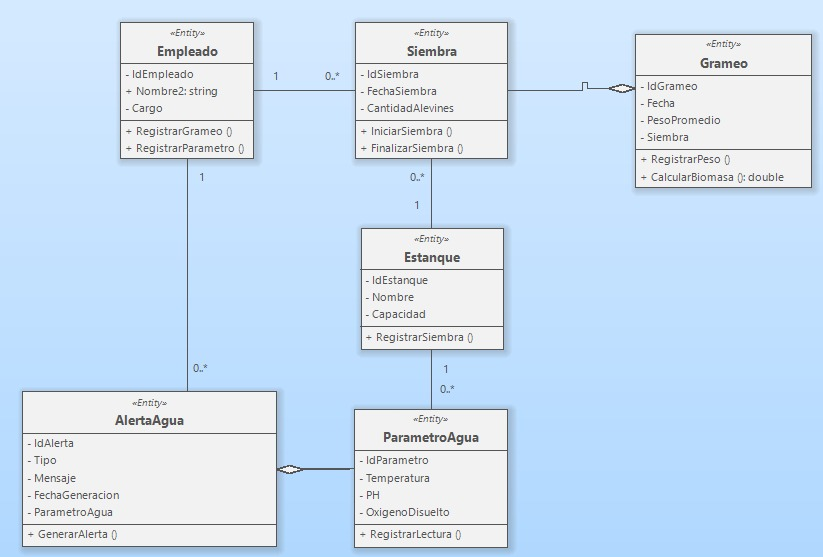
\includegraphics[width=1\textwidth]{Figura/Clases.jpeg}
    \caption{Diagrama de clases de origen -- Subsistema Control de Siembras y Monitoreo del Agua (AquaGest)}
    \label{fig:mi_imagen}
\end{figure}


\subsection{Diagramas complementarios}

Se recomienda incorporar como complemento un \textbf{diagrama de casos de uso} restringido al subsistema (Registrar Siembra, Registrar Grameo, Registrar Parámetros del Agua, Gestionar Alerta de Agua) y, si el equipo lo considera necesario para representar el comportamiento de la clase \texttt{AlertaAgua}, un \textbf{diagrama de estados} (activa \(\rightarrow\) atendida). Ambos diagramas ya cuentan con base directa en la Sección 4.1 y 4.2 del ERS de AquaGest (Figura 11 y casos de uso CU-01, CU-02).

\begin{figure}[H]
    \centering
    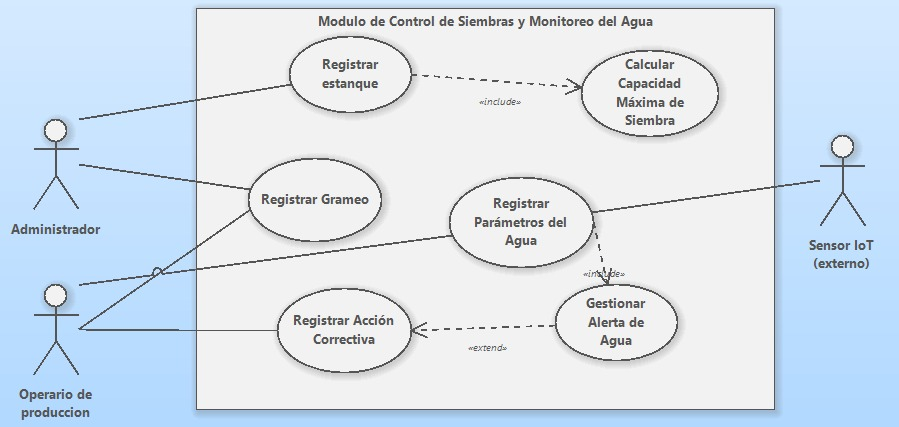
\includegraphics[width=1\textwidth]{Figura/CasoUso.jpeg}
    \caption{Diagrama de casos de uso del Subsistema de Control de Siembras y Monitoreo del Agua.}
    \label{fig:mi_imagen}
\end{figure}

\subsection{Validación de la herramienta}

Antes de ejecutar la generación, el equipo debe revisar manualmente la coherencia sintáctica y semántica del modelo dentro de Software Ideas Modeler, verificando que no existan asociaciones sin multiplicidad definida, atributos sin tipo asignado o estereotipos aplicados de forma inconsistente entre clases relacionadas. El resultado de esta revisión debe documentarse explícitamente antes de continuar con la Fase 4 (configuración del generador).

\begin{figure}[H]
    \centering
    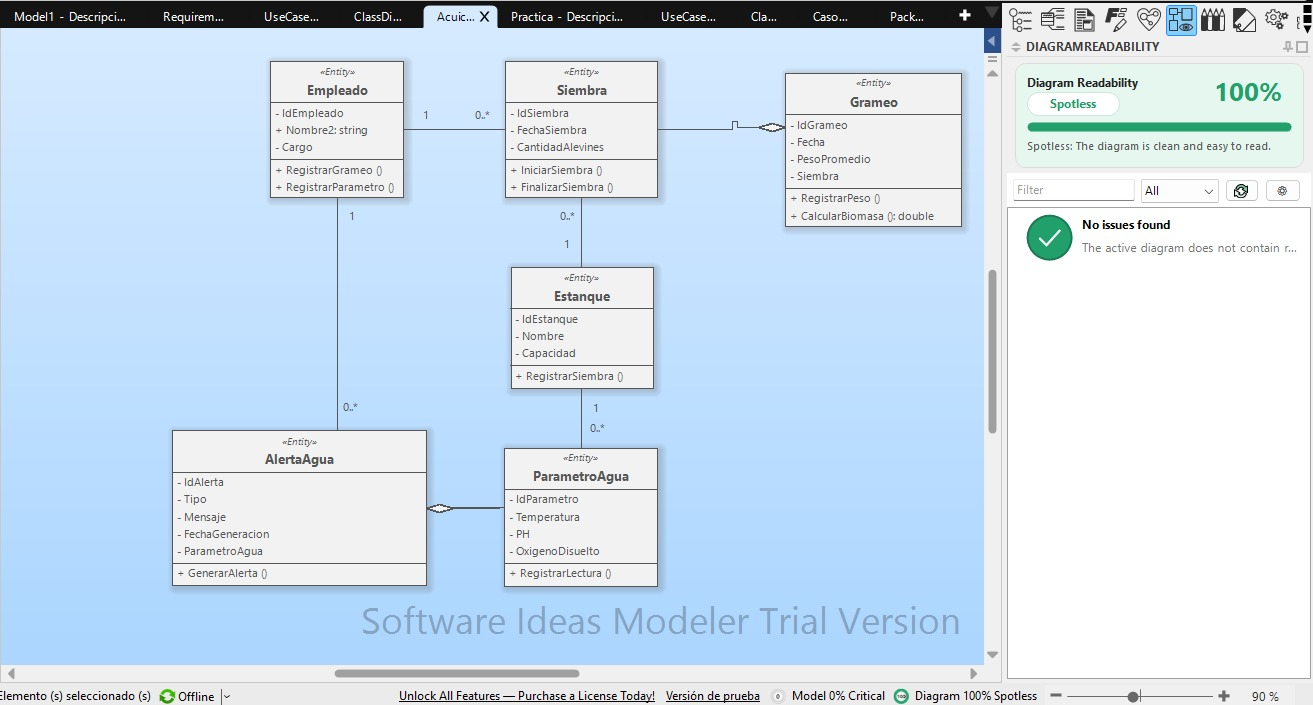
\includegraphics[width=1\textwidth]{Figura/Consistencia.jpeg}
    \caption{Revisión de consistencia del diagrama de clases del Subsistema de Control de Siembras y Monitoreo del Agua, evidenciando la ausencia de inconsistencias bloqueantes en el modelo.}
    \label{fig:mi_imagen}
\end{figure}

\subsection{Correspondencia con el archivo nativo del modelo}

El proyecto nativo de Software Ideas Modeler (\texttt{.simp}) que contiene este modelo debe conservarse como evidencia técnica junto con este documento, referenciado por su nombre de archivo y ubicación dentro del material de la actividad.

% ==================== 5. CONFIGURACIÓN DEL GENERADOR ====================
\section{Configuración del mecanismo de generación}
\label{sec:configuracion-generador}

\subsection{Plantilla y parámetros de generación}

Se utiliza el generador de código Java nativo de Software Ideas Modeler (\emph{Code Generation Templates}), configurado con los siguientes parámetros:

\begin{itemize}[leftmargin=1.4em]
    \item \textbf{Lenguaje objetivo:} Java (versión a documentar por el equipo según el JDK instalado, recomendado JDK 17 LTS).
    \item \textbf{Directorio de salida:} carpeta \texttt{generado/} dentro del material del equipo, separada de cualquier código escrito manualmente.
    \item \textbf{Organización de la salida:} creación de subcarpetas por paquete (opción \emph{Create subdirectories for packages} del asistente de generación), de forma que la estructura de directorios refleje la separación entre dominio y servicio descrita en la Sección \ref{sec:modelo-uml}.
    \item \textbf{Convención de nombres:} \texttt{PascalCase} para clases, \texttt{camelCase} para atributos y operaciones, conforme a las convenciones estándar de Java.
    \item \textbf{Política ante regeneración:} dado que Software Ideas Modeler no garantiza de forma automática la preservación de código añadido manualmente fuera de las secciones producidas por la plantilla, el equipo debe mantener claramente separado —mediante comentarios y una convención de nombres de método— el código generado del código completado a mano, y reincorporar manualmente estas adiciones tras cada regeneración (necesario para el roundtrip de la Sección \ref{sec:roundtrip}).
\end{itemize}

\subsection{Mapeo de estereotipos a construcciones del lenguaje objetivo}

La Tabla \ref{tab:mapeo-estereotipos} documenta las decisiones de mapeo entre los elementos del modelo UML y las construcciones Java que el generador de Software Ideas Modeler debe producir.

\begin{table}[H]
\centering
\caption{Mapeo de elementos del modelo a construcciones del lenguaje objetivo (Java).}
\label{tab:mapeo-estereotipos}
\begin{tabular}{p{3.2cm}p{3.2cm}p{6.5cm}}
\toprule
\textbf{Elemento del modelo} & \textbf{Estereotipo aplicado} & \textbf{Construcción Java generada} \\
\midrule
Clase de dominio (p. ej. \texttt{Estanque}) & \texttt{<<Entity>>} & Clase Java con campos privados, getters/setters y anotaciones de persistencia (a completar con el paquete ORM elegido por el equipo, p. ej. JPA). \\
Clase de lógica de negocio (p. ej. cálculo de capacidad) & \texttt{<<Service>>} & Clase Java de servicio con métodos públicos correspondientes a las operaciones del modelo. \\
Asociación 1 a 0..* (p. ej. \texttt{Estanque}--\texttt{Siembra}) & multiplicidad UML nativa & Colección tipada (\texttt{List<Siembra>}) en el lado ``muchos'' de la relación. \\
Atributo tipado (p. ej. \texttt{fecha: Date}) & tipo UML nativo & Campo Java del tipo equivalente (\texttt{java.time.LocalDate}, a definir por el equipo). \\
\bottomrule
\end{tabular}
\end{table}

\subsection{Archivos de configuración en el repositorio}

Los archivos o exportaciones de configuración de la plantilla de Software Ideas Modeler empleados en la generación deben conservarse junto al modelo nativo como parte del material técnico de la actividad, de forma que el proceso sea auditable y repetible por el docente.

\subsection{Arquitectura del código resultante}

La configuración del generador descrita en esta sección persigue que el código Java producido por Software Ideas Modeler refleje directamente las decisiones de arquitectura ya fijadas para AquaGest en su especificación de requisitos: una capa de entidades de dominio (clases con estereotipo \texttt{<<Entity>>}) desacoplada de una capa de servicios (clases con estereotipo \texttt{<<Service>>}) que expone las operaciones de negocio del subsistema. Esta separación en capas es la que posteriormente permitirá exponer el subsistema mediante una API REST consumida por el frontend web y por el módulo de inteligencia artificial, ambos externos al núcleo generado por MDD, sin que ninguno de ellos dependa de los detalles internos de persistencia de las entidades.

Adicionalmente, el equipo debe configurar en Software Ideas Modeler el paquete de destino de cada clase generada de forma que refleje esta separación (por ejemplo, un paquete \texttt{dominio} para las entidades y un paquete \texttt{servicio} para la lógica de negocio), de modo que el árbol de directorios del proyecto generado —documentado en la Sección \ref{sec:proceso-generacion}— sea legible y mantenga la trazabilidad visual entre el modelo y el código incluso para un desarrollador que no haya participado en el modelado original.

% ==================== 6. PROCESO DE GENERACIÓN ====================
\section{Proceso de generación de código}
\label{sec:proceso-generacion}

La generación se ejecuta desde Software Ideas Modeler mediante la opción de generación de código sobre el paquete que contiene el diagrama de clases validado en la Sección \ref{sec:modelo-uml}. El proceso debe documentarse con las siguientes evidencias:

\begin{figure}[H]
    \centering
    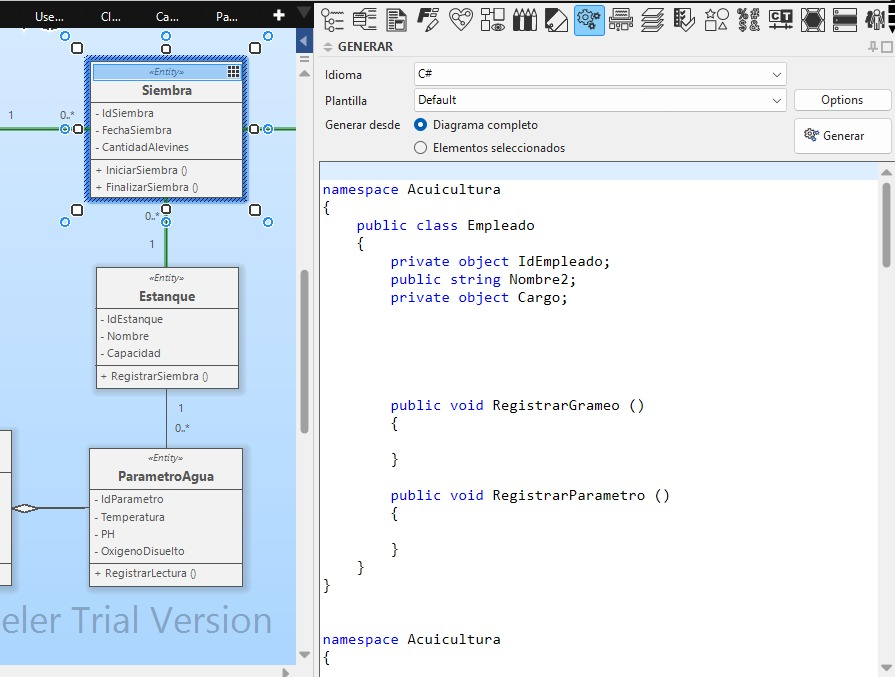
\includegraphics[width=0.8\textwidth]{Figura/GeneracionCodigo.png}
    \caption{Captura de la invocación del generador de código en Software Ideas Modeler, mostrando las clases seleccionadas y el lenguaje objetivo configurado para la generación del código fuente.}
    \label{fig:mi_imagen}
\end{figure}

\begin{figure}[H]
    \centering
    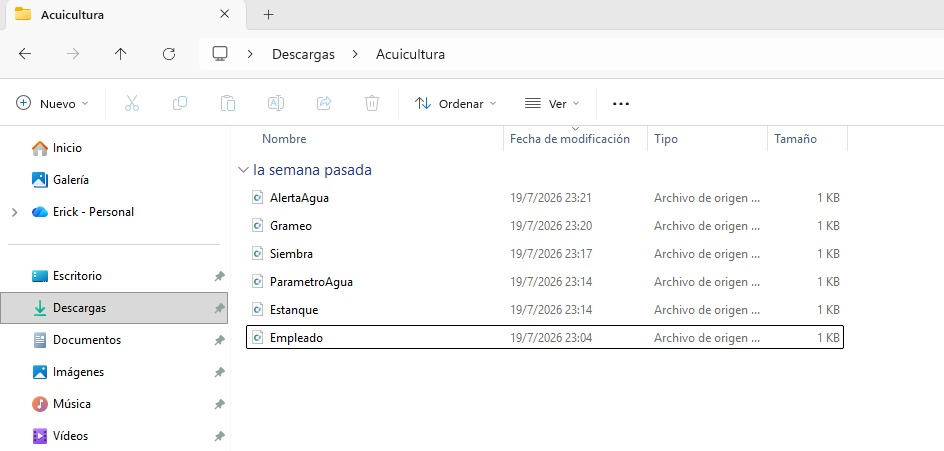
\includegraphics[width=0.8\textwidth]{Figura/CodigoGenerado.png}
    \caption{Código fuente generado automáticamente para las clases del subsistema.}
    \label{fig:mi_imagen}
\end{figure}

\begin{figure}[H]
    \centering
    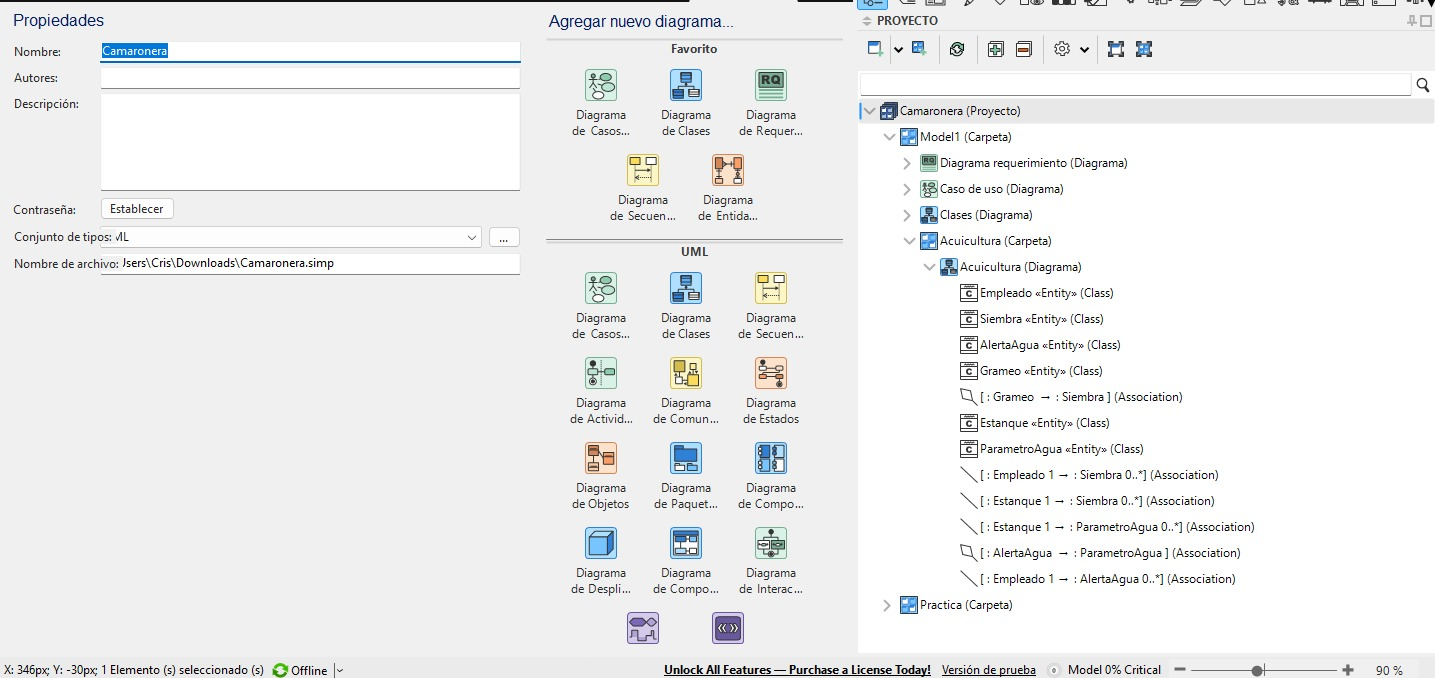
\includegraphics[width=0.8\textwidth]{Figura/ArbolPaquetes.png}
    \caption{Estructura del proyecto generado con las clases del subsistema.}
    \label{fig:mi_imagen}
\end{figure}

Se recomienda registrar también el tiempo aproximado que tomó la generación completa del subsistema, como parte de la evidencia del proceso.

% ==================== 7. VERIFICACIÓN DEL CÓDIGO GENERADO ====================
\section{Verificación del código generado}
\label{sec:verificacion}

\subsection{Apertura, compilación y ejecución de una unidad demostrable}

El proyecto generado debe abrirse en el IDE Java del equipo (IntelliJ IDEA, Eclipse o VS Code con extensión Java) y compilarse sin errores. Como unidad mínima demostrable se propone instanciar la clase \texttt{Siembra} asociada a un \texttt{Estanque} y ejecutar una operación de persistencia o una prueba unitaria simple sobre el cálculo de capacidad máxima de siembra (RF-02).

\begin{figure}[H]
    \centering
    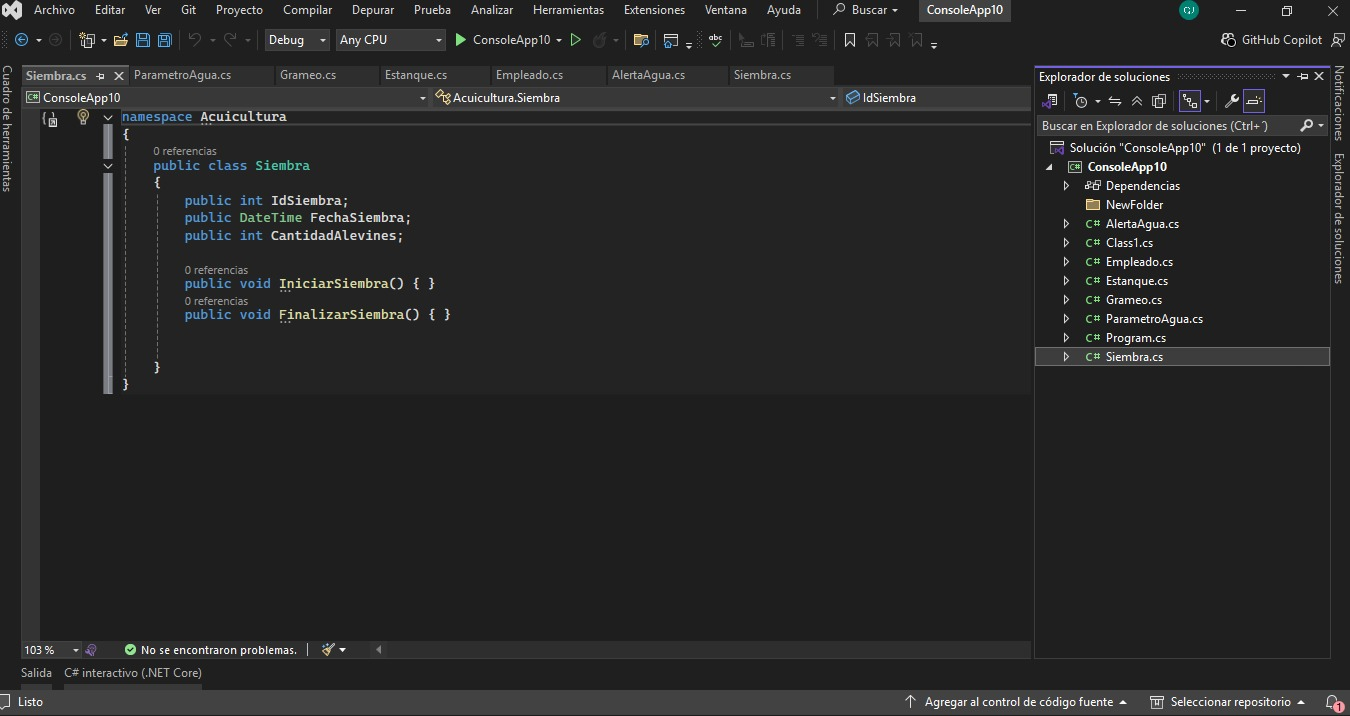
\includegraphics[width=0.8\textwidth]{Figura/Build.png}
    \caption{Compilación exitosa del proyecto generado en Visual Studio, sin errores de construcción.}
    \label{fig:mi_imagen}
\end{figure}

\subsection{Correspondencia modelo \(\rightarrow\) código}

La Tabla \ref{tab:correspondencia} documenta la trazabilidad entre los elementos del modelo UML y los artefactos de código efectivamente generados. Esta tabla debe completarse con los nombres reales de archivo una vez ejecutada la generación.

\begin{table}[H]
\centering
\caption{Correspondencia modelo \(\rightarrow\) código generado (plantilla a completar por el equipo).}
\label{tab:correspondencia}
\begin{tabular}{p{2.6cm}p{2.6cm}p{2.6cm}p{4.7cm}}
\toprule
\textbf{Clase UML} & \textbf{Atributo/Operación} & \textbf{Archivo generado} & \textbf{Campo/método Java} \\
\midrule
\texttt{Estanque} & \texttt{codigo: String} & \emph{a completar} & \emph{a completar} \\
\texttt{Siembra} & \texttt{registrarSiembra()} & \emph{a completar} & \emph{a completar} \\
\texttt{ParametroAgua} & \texttt{valor: Decimal} & \emph{a completar} & \emph{a completar} \\
\texttt{AlertaAgua} & \texttt{estado: String} & \emph{a completar} & \emph{a completar} \\
\bottomrule
\end{tabular}
\end{table}

\subsection{Limitaciones observadas del generador}

Tras ejecutar la generación real del codigo fuente, qué elementos del modelo \emph{no} fueron generados automáticamente y requirieron completarse a mano (por ejemplo: lógica de validación de negocio compleja como la comparación contra rangos óptimos de RF-10, configuración del \texttt{persistence.xml}, o la conexión efectiva a PostgreSQL/MySQL). El código escrito manualmente debe distinguirse claramente del código generado mediante carpetas separadas, comentarios o marcadores de bloque protegido.

\begin{figure}[H]
    \centering
    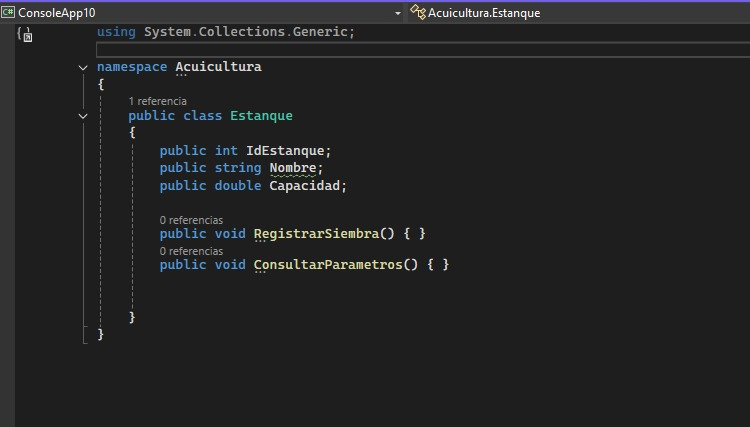
\includegraphics[width=0.8\textwidth]{Figura/CodigoIncopleto.png}
    \caption{Código fuente generado automáticamente para la clase \texttt{Estanque} antes de incorporar las relaciones definidas en el diagrama UML.}
    \label{fig:mi_imagen}
\end{figure}

\begin{figure}[H]
    \centering
    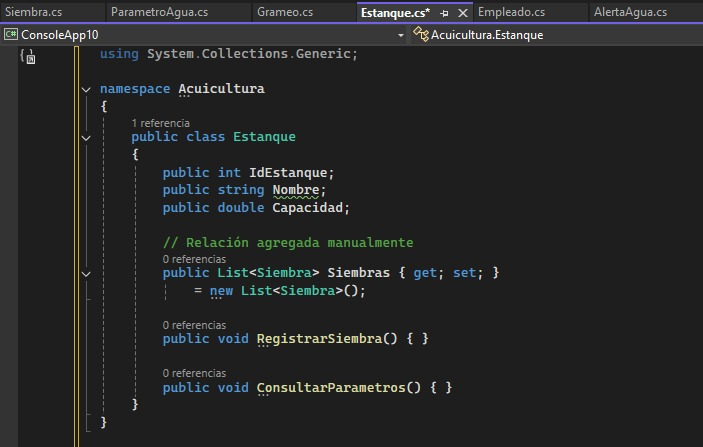
\includegraphics[width=0.8\textwidth]{Figura/CodigoManual.png}
    \caption{Código fuente de la clase \texttt{Estanque} después de añadir manualmente las relaciones UML no generadas por la herramienta.}
    \label{fig:mi_imagen}
\end{figure}

\subsection{Verificación frente a requisitos no funcionales relacionados}

Si bien la actividad se concentra en la verificación funcional del código generado, conviene relacionar el resultado con los requisitos no funcionales del ERS de AquaGest que el subsistema modelado debe respetar una vez integrado al resto del sistema. En particular, el tiempo de registro de un parámetro del agua (RNF-01, tiempo de respuesta no mayor a 2 segundos) y la política de control de acceso basado en roles (RNF-04) condicionan decisiones que exceden lo que el generador de Software Ideas Modeler produce automáticamente: la primera exige que la capa de persistencia generada se acompañe de un mecanismo de conexión eficiente a la base de datos relacional, y la segunda exige incorporar manualmente la lógica de autenticación y autorización sobre los servicios generados. El equipo debe dejar constancia de que estas verificaciones de calidad quedan pendientes de una fase de pruebas no funcionales posterior a esta actividad, y no deben confundirse con la verificación funcional mínima exigida en la Sección \ref{sec:verificacion}.

% ==================== 8. CIERRE DEL CICLO (ROUNDTRIP) ====================
\section{Cierre del ciclo: roundtrip controlado}
\label{sec:roundtrip}

Para evidenciar el cierre completo del ciclo MDD, se ejecuta un cambio no trivial sobre el modelo de origen: se propone agregar el atributo \texttt{observaciones: String} a la clase \texttt{Grameo} (permitiendo registrar notas cualitativas del muestreo semanal, tal como se documentó en el hallazgo 3 de la entrevista con el Técnico Acuícola, Apéndice B.3 del ERS) o, alternativamente, modificar la cardinalidad de la relación \texttt{Estanque}--\texttt{AlertaAgua} si el equipo detecta una inconsistencia durante el modelado.

\subsection{Procedimiento}

\begin{enumerate}[leftmargin=1.6em]
    \item Se captura el estado \emph{antes} del modelo (diagrama de clases) y del código generado para la clase afectada.
    \item Se aplica el cambio directamente sobre el diagrama de clases en Software Ideas Modeler.
    \item Se regenera el código para la clase afectada y se reincorpora manualmente, sobre el nuevo código, cualquier adición que se hubiese completado a mano en la Sección \ref{sec:verificacion}, siguiendo la convención de separación documentada en la Sección \ref{sec:configuracion-generador}.
    \item Se captura el estado \emph{después} del modelo y del código regenerado, verificando que el cambio se refleje correctamente y que la reincorporación del código manual se haya realizado sin pérdida de información.
\end{enumerate}

\begin{figure}[H]
    \centering
    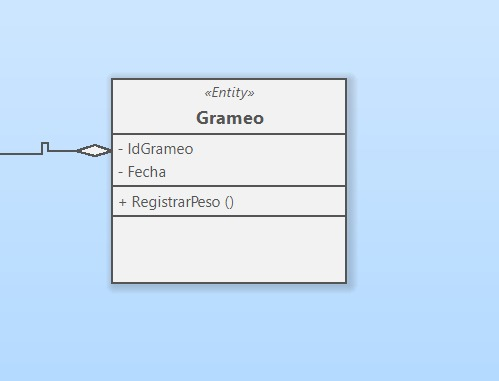
\includegraphics[width=0.5\textwidth]{Figura/GrameoAntes.png}
\caption{Diagrama de clases de la clase \texttt{Grameo} antes de incorporar el atributo \texttt{Observaciones} en el modelo UML.}
    \label{fig:mi_imagen}
\end{figure}

\begin{figure}[H]
    \centering
    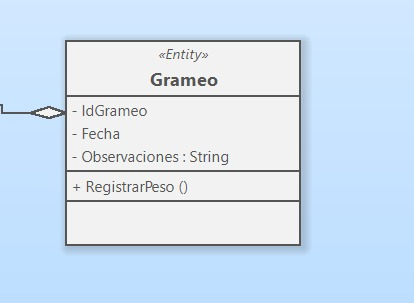
\includegraphics[width=0.5\textwidth]{Figura/GrameoDespues.png}
\caption{Diagrama de clases de la clase \texttt{Grameo} después de incorporar el atributo \texttt{Observaciones} en el modelo UML.}
    \label{fig:mi_imagen}
\end{figure}

\begin{figure}[H]
    \centering
    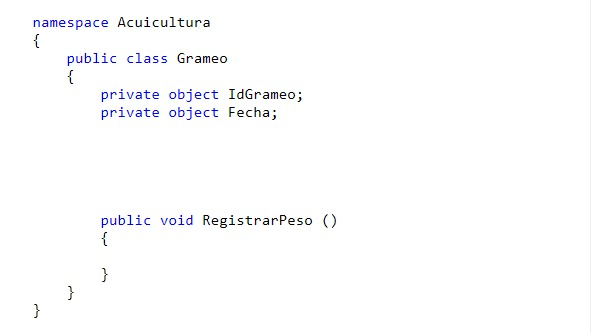
\includegraphics[width=0.8\textwidth]{Figura/CodGrameoAntes.png}
\caption{Código fuente generado para la clase \texttt{Grameo} antes de la regeneración del modelo.}
    \label{fig:mi_imagen}
\end{figure}

\begin{figure}[H]
    \centering
    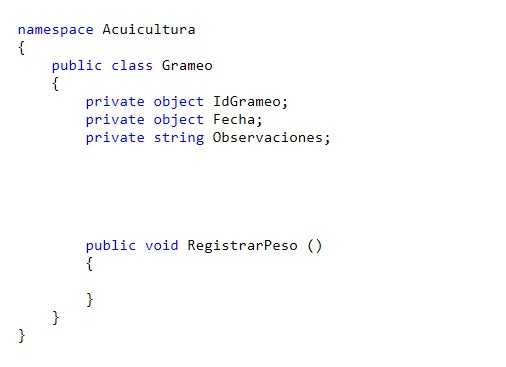
\includegraphics[width=0.8\textwidth]{Figura/CodGrameoDespues.png}
\caption{Código fuente de la clase \texttt{Grameo} después de la regeneración, incorporando el atributo \texttt{Observaciones} definido en el modelo UML.}
    \label{fig:mi_imagen}
\end{figure}

\subsection{Manejo del código completado manualmente}

Software Ideas Modeler no garantiza de forma automática la preservación de código añadido manualmente fuera de lo producido por la plantilla al ejecutar una nueva generación; por ello, la disciplina de separación (comentarios, convención de nombres) definida en la Sección \ref{sec:configuracion-generador} es la que permite al equipo identificar con certeza qué fragmentos deben reincorporarse tras cada regeneración. El equipo debe documentar aquí, con evidencia real, el procedimiento seguido para reincorporar el código manual añadido en la Sección \ref{sec:verificacion} tras ejecutar este roundtrip, y si se detectó alguna pérdida de información en el proceso.

\subsection{Implicaciones del roundtrip para el ciclo de vida de AquaGest}

Más allá de su función demostrativa dentro de esta actividad, el roundtrip documentado en esta sección anticipa un patrón de trabajo que el equipo deberá sostener durante el resto del desarrollo del PFC AquaGest: cada vez que la especificación de requisitos evolucione —por ejemplo, si durante las pruebas con el administrador de la Compañía Biofina surge la necesidad de registrar un nuevo atributo en el historial de grameos, o de ajustar la cardinalidad de la relación entre \texttt{Siembra} y \texttt{Cosecha}— el cambio debería introducirse primero en el modelo de Software Ideas Modeler y propagarse después al código mediante regeneración, en lugar de aplicarse directamente sobre las clases Java ya generadas. Este patrón de trabajo es el que permite que el modelo conserve su condición de fuente autoritativa del sistema a lo largo de todo el proyecto, y no únicamente durante la actividad de generación inicial documentada en este informe. Sostener esta disciplina exige, sin embargo, que el equipo delimite con claridad —mediante la convención de separación descrita en la Sección \ref{sec:configuracion-generador}— qué porciones del código generado pueden completarse manualmente y reincorporarse tras cada regeneración, y cuáles deben permanecer exclusivamente bajo control del modelo.

% ==================== 9. CONCLUSIONES ====================
\section{Conclusiones}
\label{sec:conclusiones}

La aplicación del ciclo MDD sobre el subsistema de Control de Siembras y Monitoreo del Agua de AquaGest permitió comprobar, a nivel conceptual y operativo, que el modelo de clases ya validado en el ERS del proyecto constituye una base directamente aprovechable para la generación de código, siempre que se complemente con los estereotipos y perfiles necesarios para que el generador de Software Ideas Modeler produzca las construcciones esperadas del lenguaje objetivo. El enfoque MDD aporta valor real al PFC en tres frentes concretos: (i) reduce el esfuerzo de escritura manual de código repetitivo (entidades, getters/setters, esqueletos de servicio); (ii) refuerza la trazabilidad entre los requisitos funcionales formalizados (RF-01 a RF-10) y el código resultante, mediante la tabla de correspondencia de la Sección \ref{sec:verificacion}; y (iii) evidencia, mediante el roundtrip de la Sección \ref{sec:roundtrip}, que el modelo puede mantenerse como fuente autoritativa incluso después de iniciada la implementación.

Como limitación general del enfoque, se anticipa que la lógica de negocio compleja del dominio acuícola —en particular las reglas de alerta por parámetros fuera de rango (RF-10) y el cálculo de eficiencia alimenticia (RF-14)— excede lo que un generador basado en plantillas puede producir automáticamente, por lo que dicha lógica deberá completarse manualmente y reincorporarse tras cada regeneración del código, siguiendo la convención de separación documentada en la Sección \ref{sec:configuracion-generador}. Asimismo, el alcance de esta actividad se limitó a un subsistema representativo (seis clases del dominio); la extensión del mismo enfoque al resto de los módulos de AquaGest (Alimentación, Historial Sanitario, Inventario, Cosechas) queda como trabajo futuro natural hacia las siguientes fases de implementación del PFC, una vez consolidado el modelo de dominio completo.

Finalmente, la experiencia documentada en este ejercicio deja tres lecciones aprovechables para el resto del desarrollo de AquaGest. Primero, que mantener el diagrama de clases en Software Ideas Modeler como fuente única de verdad del modelo de dominio —en lugar de dejar que diverja del código a medida que este evolucione— exige disciplina de equipo: cada cambio estructural relevante debería originarse en el modelo y propagarse mediante regeneración, no aplicarse directamente y de forma definitiva sobre el código generado sin reincorporarlo tras el siguiente ciclo de generación. Segundo, que la inversión inicial de tiempo en tipar correctamente los atributos, definir con precisión las multiplicidades y aplicar los estereotipos adecuados se traduce directamente en menor esfuerzo de corrección posterior sobre el código generado, lo que confirma en la práctica la relación entre calidad del modelo y calidad del artefacto derivado discutida en el marco teórico de este documento (Sección \ref{sec:marco-teorico}). Tercero, que el enfoque MDD no sustituye la necesidad de pruebas de verificación funcional y no funcional sobre el sistema final, sino que desplaza parte del esfuerzo de desarrollo desde la escritura repetitiva de código hacia el diseño cuidadoso del modelo, lo cual resulta especialmente valioso para un equipo académico con tiempo limitado como el que desarrolla el PFC AquaGest.

% ==================== REFERENCIAS ====================
\newpage
\bibliographystyle{ieeetr}
\bibliography{referencias}
\addcontentsline{toc}{section}{Referencias}

% ==================== ANEXO ====================
\newpage
\appendix
\section{Anexo: correspondencia con la especificación de requisitos de AquaGest}

La Tabla \ref{tab:anexo-rf} resume la relación entre los requisitos funcionales del ERS de AquaGest cubiertos por el subsistema modelado en este documento y el elemento del modelo UML que los materializa.

\begin{table}[H]
\centering
\caption{Requisitos funcionales del ERS de AquaGest cubiertos por el subsistema modelado.}
\label{tab:anexo-rf}
\begin{tabular}{p{1.6cm}p{6.5cm}p{4.2cm}}
\toprule
\textbf{RF} & \textbf{Descripción (ERS AquaGest)} & \textbf{Elemento del modelo UML} \\
\midrule
RF-01 & Registro de estanque & Clase \texttt{Estanque} \\
RF-02 & Cálculo de capacidad máxima de siembra & Operación en clase \texttt{Estanque} / \texttt{<<Service>>} \\
RF-04 & Actualización de estado del estanque & Atributo \texttt{estado} en \texttt{Estanque} \\
RF-05 & Registro de siembra & Clase \texttt{Siembra} \\
RF-06 & Registro de grameo semanal & Clase \texttt{Grameo} \\
RF-09 & Registro de parámetros del agua & Clase \texttt{ParametroAgua} \\
RF-10 & Alerta por parámetro fuera de rango & Clase \texttt{AlertaAgua} \\
\bottomrule
\end{tabular}
\end{table}

La Tabla \ref{tab:anexo-rnf} complementa la anterior indicando los requisitos no funcionales del proyecto AquaGest que, si bien no son generados automáticamente por Software Ideas Modeler, condicionan directamente las decisiones de configuración tomadas en la Sección \ref{sec:configuracion-generador} sobre el código derivado del subsistema modelado.

\begin{table}[H]
\centering
\caption{Requisitos no funcionales relacionados con el subsistema modelado.}
\label{tab:anexo-rnf}
\begin{tabular}{p{1.8cm}p{6.5cm}p{4.0cm}}
\toprule
\textbf{RNF} & \textbf{Descripción (ERS AquaGest)} & \textbf{Relación con el código generado} \\
\midrule
RNF-01 & Eficiencia de desempeño: registro de un parámetro del agua en no más de 2 segundos bajo carga normal & Exige una capa de persistencia eficiente sobre las entidades \texttt{ParametroAgua} y \texttt{AlertaAgua} generadas \\
RNF-02 & Disponibilidad del sistema de al menos el 98\,\% del tiempo mensual & Motiva el desacoplamiento de capas (dominio/servicio) reflejado en el paquete generado \\
RNF-04 & Seguridad: control de acceso basado en roles (RBAC) y cifrado de contraseñas & Debe incorporarse manualmente sobre los servicios generados; no forma parte de la plantilla de generación estructural \\
\bottomrule
\end{tabular}
\end{table}

\end{document}
